% Compile with Tectonic/XeLaTeX.
\documentclass[10pt,a4paper]{article}

\usepackage[a4paper,margin=1.45cm]{geometry}
\usepackage{fontspec}
\IfFileExists{/System/Library/Fonts/Supplemental/Arial.ttf}{
  \setmainfont[
    Path=/System/Library/Fonts/Supplemental/,
    UprightFont={Arial.ttf},
    BoldFont={Arial Bold.ttf},
    ItalicFont={Arial Italic.ttf},
    BoldItalicFont={Arial Bold Italic.ttf}
  ]{Arial}
  \setsansfont[
    Path=/System/Library/Fonts/Supplemental/,
    UprightFont={Arial.ttf},
    BoldFont={Arial Bold.ttf},
    ItalicFont={Arial Italic.ttf},
    BoldItalicFont={Arial Bold Italic.ttf}
  ]{Arial}
}{
  \IfFontExistsTF{Times New Roman}{\setmainfont{Times New Roman}}{\setmainfont{TeX Gyre Termes}}
  \IfFontExistsTF{Arial}{\setsansfont{Arial}}{\setsansfont{TeX Gyre Heros}}
}
\usepackage{graphicx}
\usepackage{booktabs}
\usepackage{adjustbox}
\usepackage{tabularx}
\usepackage{array}
\usepackage{enumitem}
\usepackage{xcolor}
\usepackage{hyperref}
\usepackage{caption}
\usepackage{subcaption}
\usepackage{float}
\usepackage{amsmath}
\usepackage{xurl}

\graphicspath{{../outputs/figures/}{outputs/figures/}}
\hypersetup{colorlinks=true,linkcolor=black,urlcolor=blue,citecolor=black}
\setlength{\parskip}{3pt}
\setlength{\parindent}{0pt}
\setlist[itemize]{leftmargin=1.15em,itemsep=1pt,topsep=2pt}
\setlist[enumerate]{leftmargin=1.30em,itemsep=1pt,topsep=2pt}
\captionsetup{font=small,labelfont=bf}
\renewcommand{\arraystretch}{1.10}
\renewcommand{\figurename}{Hình}
\renewcommand{\tablename}{Bảng}
\emergencystretch=4em

\newcommand{\code}[1]{\texttt{#1}}
\newcommand{\TenDeTai}{ODA-based Multi-sensor Risk-aware UAV Obstacle Avoidance Benchmark}
\newcommand{\SinhVien}{Nguyễn Thanh Lâm}
\newcommand{\Mentor}{Lê Trung Kiên}
\newcommand{\DonViMentor}{Viettel High Tech}
\newcommand{\EmailMentor}{kienlt23@gmail.com}

\begin{document}

\begin{center}
{\Large\bfseries \TenDeTai}\\[3pt]
{\large\bfseries Báo cáo tiến độ kỹ thuật}\\[4pt]
{\normalsize \SinhVien, \Mentor\textsuperscript{1}}\\
{\small \textsuperscript{1}\DonViMentor}\\[3pt]
{\small Cập nhật đến ngày 02/07/2026}
\end{center}

\section*{Tóm tắt kỹ thuật}

Trọng tâm chính của đề tài là ODA Dataset cho bài toán UAV obstacle avoidance; các dataset ngoài ODA chỉ dùng để stress-test perception/LiDAR. Pipeline hiện đọc metadata, OptiTrack, RGB video, radar và IMU; tạo risk label từ clearance; so sánh planner; cache monocular depth; huấn luyện baseline future-risk; xử lý point cloud thật để xuất 3D bounding box; bổ sung demo ROS2/Gazebo fused costmap; dựng demo Isaac Sim RGB-D/LiDAR indoor; mở rộng lên hướng full 3D voxel/ESDF với MPPI trong không gian \(x,y,z\); và thêm thí nghiệm online latency cho LiDAR 3D 10 Hz.

Về bản chất, báo cáo không chỉ trình bày một demo bay tránh vật cản, mà xây dựng một chuỗi đánh giá có thể đo được: dùng ground truth để định nghĩa nguy cơ va chạm, dùng planner để kiểm tra mức độ khó của bài toán hình học, rồi đưa RGB/radar/IMU/LiDAR vào như các nguồn cảm biến để tiến dần tới perception-driven planning.

\begin{table}[H]
\centering
\small
\caption{Kết quả tiến độ chính.}
\begin{tabularx}{0.98\linewidth}{>{\bfseries}p{3.5cm} X}
\toprule
Hạng mục & Trạng thái/Kết quả \\
\midrule
ODA benchmark & 300/300 target trials ready; 150 trial một vật cản và 150 trial hai vật cản. \\
Planner comparison & Báo cáo giữ lại 1800 dòng metric trên 300 trial cho các planner được trình bày; RRT và RRT* đạt 0 collision và 0 safety violation; MPPI đạt collision 0, violation 0.0033. \\
Perception-risk & 50 ODA trial, 2584 frame feature; Depth Anything V2 Small + radar + IMU; split theo trial ID. \\
Depth timing & Depth Anything V2 Small: 0.063874 s/frame wall-time, 0.017378 s/frame inference-time, batch size 8. \\
LiDAR processing & Multi-LiDAR HolybroStdn01, Tello03, TelloOut02: ground removal, voxel clustering, 3D AABB thật trên Ouster/Mid360/Avia. \\
3D/fusion demo & Three.js demo có source grid PointCloud2/LiDAR/depth và fused occupancy grid; ROS2/Gazebo fused-costmap runtime đã pass 13/13 topics, 13/13 message samples và costmap mux. \\
Full 3D ESDF/MPPI & Synthetic indoor 3D voxel map \(\rightarrow\) ESDF \(\rightarrow\) MPPI \(x,y,z\); collision 0, safety violation 0. Server đã verify PointCloud2 LiDAR \(\rightarrow\) local 3D ESDF \(\rightarrow\) MPPI, đồng thời NVBlox chạy TSDF/ESDF runtime. \\
Online latency 10 Hz & Thí nghiệm hẹp theo câu hỏi mentor: LiDAR period \(100\,ms\), map/ESDF update \(5.9\,ms\), MPPI \(28.9\)--\(205.5\,ms\), tổng delay \(144.7\)--\(321.4\,ms\) cho UAV \(1\)--\(6\,m/s\). Bảng synthetic chỉ là kinematic latency proxy để đo delay distance và clearance; bổ sung 144 case online 10 Hz cho RRT, RRT* và MPPI qua 8 seed/case mỗi tốc độ; thêm ODA replay 3D 384 case dùng OptiTrack pose tại \(t+T_{\mathrm{delay}}\). \\
Sensor frontend latency & Bổ sung timing sensor-to-occupancy: ODA cached depth-to-grid \(2.3\,ms\), ODA Depth Anything V2 Small-to-grid \(66.2\,ms\), external LiDAR bbox-to-grid \(0.02\,ms\); camera/depth 5 fps chỉ safe tới khoảng \(2\,m/s\) trong delay check này. \\
Isaac Sim sensor demo & Headless Isaac Sim 6.0.1 trên RTX 4090; video 1920\(\times\)1080, 180 frame/10 s; RGB-D từ Replicator, LiDAR/point-cloud panel từ geometry raycast, dynamic indoor obstacles; min clearance \(0.3225\,m\), collision 0. \\
Đầu ra báo cáo & CSV metrics, PNG figures, MP4 qualitative videos, Hugging Face dataset/result backup, PDF technical report. \\
Audit local 01/07/2026 & \code{audit\_progress\_submission.py} pass toàn bộ PDF/video/artifact; \code{check\_perception\_to\_planner\_contract.py} và \code{check\_perception\_planner\_matrix.py} pass bằng \code{.venv}; \code{compileall} pass cho source Python. \\
\bottomrule
\end{tabularx}
\end{table}

\section{Mục tiêu và phạm vi}

\textbf{Mục tiêu giai đoạn hiện tại:} tạo benchmark nhẹ, có số liệu và có minh chứng hình ảnh cho UAV obstacle avoidance trên ODA.

\textbf{Phạm vi thực hiện:}
\begin{itemize}
  \item Xử lý CSV/metadata/ground truth trước; ROS/Gazebo chỉ là nhánh demo runtime, chưa thay thế pipeline benchmark chính.
  \item Đánh giá an toàn bằng metric hình học từ OptiTrack và obstacle metadata.
  \item So sánh planner classical baseline trước khi mở rộng perception-risk.
  \item Dùng LiDAR external dataset để chứng minh năng lực point-cloud processing, không thay thế ODA benchmark.
\end{itemize}

\textbf{Các claim không đưa ra ở giai đoạn này:}
\begin{itemize}
  \item Monocular depth chưa phải metric depth theo mét.
  \item Dynamic feasibility hiện gồm smoothness proxy 2D và online latency/kinematic delay check 3D, chưa phải full quadrotor dynamics hoặc actuator-constrained control.
  \item TensorRT chưa có engine thật do thiếu runtime \code{trtexec}/\code{libnvinfer} trên container đã dùng.
  \item PX4/offboard chưa runtime-verified trên server hiện tại vì thiếu PX4 SITL, \code{px4\_msgs} và Micro XRCE bridge.
  \item NVBlox 3D runtime và PointCloud2 LiDAR \(\rightarrow\) local 3D ESDF \(\rightarrow\) MPPI đã verify; chưa claim direct query toàn bộ NVBlox 3D ESDF volume hoặc closed-loop PX4/offboard.
  \item Isaac Sim demo mới là sensor/planner visualization: RGB-D từ Isaac Replicator, LiDAR panel là point cloud raycast từ hình học scene; chưa claim RTX LiDAR API hoặc PX4 closed-loop.
\end{itemize}

\section{Định nghĩa bài toán}

\textbf{Bài toán chính:} với một trial bay của MAV trong môi trường indoor có vật cản, sử dụng dữ liệu đa cảm biến và ground truth để (i) đánh giá mức độ an toàn của quỹ đạo đã bay, (ii) so sánh các planner tránh vật cản trên cùng điều kiện start/goal/obstacle, và (iii) tạo feature perception-risk để dự đoán nguy cơ trong tương lai gần.

\begin{table}[H]
\centering
\small
\caption{Định nghĩa input/output của bài toán trong giai đoạn hiện tại.}
\begin{tabularx}{0.98\linewidth}{>{\bfseries}p{3.2cm} X}
\toprule
Thành phần & Định nghĩa \\
\midrule
Input chính & Mỗi trial ODA gồm OptiTrack trajectory của MAV, metadata vị trí vật cản, video RGB, radar CSV và IMU CSV. \\
Không gian đánh giá & Mặt phẳng bay 2D \(x-z\) từ OptiTrack; chiều cao \(y\) chưa dùng trong planner benchmark hiện tại. \\
Obstacle model & Vật cản được mô hình hóa bằng circle/cylinder footprint bán kính \(r=0.20\,m\), kèm safety clearance \(0.50\,m\). \\
Output an toàn & Minimum clearance, collision flag, safety-distance violation flag, closest-approach time, risk label theo thời gian. \\
Output planner & Quỹ đạo ứng viên từ straight-line, geometric bypass, RRT, RRT*, MPPI; so sánh bằng collision, violation, clearance, length, smoothness, compute time. \\
Output perception-risk & Feature depth/radar/IMU theo frame và nhãn \code{future\_risk\_label} để đánh giá khả năng cảnh báo sớm. \\
\bottomrule
\end{tabularx}
\end{table}

\textbf{Formulation rút gọn:} cho quỹ đạo \(\tau=\{\mathbf{p}_0,\ldots,\mathbf{p}_T\}\), tập vật cản \(\mathcal{O}=\{\mathbf{o}_1,\ldots,\mathbf{o}_K\}\), planner cần sinh đường đi từ start đến goal sao cho tránh vùng vật cản đã inflate bởi \(r+0.50\,m\). Bài toán đánh giá không tối ưu trực tiếp trên UAV dynamics, mà đo:
\[
\min_t c_t,\quad \mathbf{1}[\min_t c_t<0],\quad \mathbf{1}[\min_t c_t<0.50],\quad L(\tau),\quad S(\tau),\quad T_{\mathrm{compute}},
\]
trong đó \(c_t\) là clearance tới biên vật cản, \(L(\tau)\) là path length, \(S(\tau)\) là smoothness proxy, và \(T_{\mathrm{compute}}\) là thời gian tính planner.

\textbf{Phạm vi bài toán phụ:} LiDAR external dataset không được dùng để tính metric tránh vật cản của ODA. Nó được dùng để kiểm chứng một bài toán perception riêng: từ point cloud thật, tách foreground cluster và xuất 3D bounding box cho obstacle-like structures.

\section{Dữ liệu và chuẩn bị thí nghiệm}

\begin{table}[H]
\centering
\small
\caption{Nguồn dữ liệu đã dùng.}
\begin{tabularx}{0.98\linewidth}{>{\bfseries}p{3.3cm} p{3.5cm} X}
\toprule
Nguồn & Vai trò & Nội dung đã xử lý \\
\midrule
ODA Dataset & Benchmark chính & Metadata, OptiTrack trajectory, RGB video, radar CSV, IMU CSV; chọn 300 trial mục tiêu. \\
Multi-LiDAR & LiDAR stress-test & Calibration, HolybroStdn01, Tello03, TelloOut02; Ouster PointCloud2, Livox Mid360/Avia CustomMsg. \\
ARCO Dataset & Point-cloud reference & ROS2 bag sample với Ouster point cloud; dùng để kiểm tra parser/segmentation ngoài ODA. \\
Hugging Face Hub & Lưu trữ dữ liệu/kết quả & Upload raw rosbag nén \code{.zst}, checksum và output tables/figures. \\
\bottomrule
\end{tabularx}
\end{table}

\begin{table}[H]
\centering
\small
\caption{Quy mô ODA đã khai thác.}
\begin{tabular}{lr}
\toprule
Chỉ số & Giá trị \\
\midrule
Trial ID trong metadata & 1369 \\
Dòng \code{trial\_overview.csv} & 1997 \\
Trial full-light + video + obstacle hợp lệ & 1108 \\
Target benchmark đã extract & 300/300 \\
Planner metric rows & 2100 \\
Depth/radar/IMU feature rows & 2584 \\
\bottomrule
\end{tabular}
\end{table}
{\small \emph{Ghi chú:} với bảng LiDAR, dấu $\uparrow*$ nghĩa là nhiều điểm/cụm/bbox hơn, tức nhiều evidence obstacle hơn; không phải luôn tốt tuyệt đối nếu nhiễu hoặc over-segmentation cao.}

\section{Pipeline triển khai}

\begin{table}[H]
\centering
\small
\caption{Các module/script chính và đầu ra.}
\begin{tabularx}{0.98\linewidth}{>{\bfseries}p{4.0cm} X}
\toprule
Nhóm xử lý & Chức năng và output \\
\midrule
ODA ingestion & Đọc metadata/OptiTrack/radar/IMU/video; tạo readiness manifest 20/50/100/300 trial. \\
Safety metrics & Minimum distance, boundary clearance, collision, safety violation, closest approach, path length, smoothness, compute time. \\
Planner benchmark & Human, straight-line, geometric bypass, RRT, RRT*, MPPI; output \code{planner\_comparison\_summary\_300.csv}. \\
Qualitative video & RGB, relative depth, radar FFT, IMU, safety map, trajectory; output MP4 và contact sheet. \\
Perception-risk & Depth/radar/IMU features, future-risk label, imbalance-aware threshold tuning. \\
LiDAR segmentation & ROS bag parser without ROS runtime, ROI crop, ground removal, voxel clustering, 3D AABB export. \\
\bottomrule
\end{tabularx}
\end{table}

\clearpage

\section{Bản chất phương pháp}

Phần nền motion planning được hiểu theo khung trong \textit{Modern Robotics}: robot có trạng thái/cấu hình, môi trường có vùng cấm do vật cản tạo ra, và planner phải tìm đường từ start đến goal sao cho không đi qua vùng va chạm \cite{modernRobotics}. Trong báo cáo này, bài toán được rút gọn trước về mặt phẳng bay \(x-z\) để có benchmark chắc chắn, sau đó mới mở rộng sang voxel/ESDF 3D.

\begin{table}[H]
\centering
\small
\caption{Bản chất các khối phương pháp trong báo cáo.}
\begin{tabularx}{0.98\linewidth}{>{\bfseries}p{3.1cm} X X}
\toprule
Khối & Bản chất kỹ thuật & Cách hiểu khi báo cáo cấp trên \\
\midrule
Ground truth ODA & OptiTrack và obstacle metadata cho biết MAV đã bay ở đâu và vật cản nằm ở đâu. Từ đó tính được clearance thật theo hình học, không phụ thuộc vào model perception. & Đây là phần biến dataset thành benchmark định lượng, không chỉ là video minh họa. \\
Safety/risk label & Collision là khi clearance âm; safety violation là khi clearance nhỏ hơn ngưỡng an toàn. Future-risk dùng horizon ngắn để biến clearance sắp tới thành nhãn cảnh báo. & Metric an toàn là cơ sở chung để so sánh người lái, planner và perception-risk. \\
Planner 2D & RRT/RRT* lấy mẫu trong không gian bay \cite{rrt,rrtstar}; MPPI lấy nhiều rollout và chọn trajectory có cost thấp \cite{mppi}. & Nếu biết bản đồ vật cản, bài toán hình học hiện đã giải được khá tốt; thách thức thực tế chuyển sang sensing, mapping và control. \\
Perception-risk & RGB depth chỉ là relative depth, radar cho range-Doppler cue, IMU cho trạng thái chuyển động; classifier học mối liên hệ giữa các cue này và nhãn future-risk \cite{depthAnythingV2,tiRadar}. & Đây là bước từ ground-truth benchmark sang cảnh báo sớm dựa trên cảm biến. Chưa claim depth theo mét nếu chưa hiệu chuẩn. \\
LiDAR segmentation & Point cloud được crop/voxel hóa, loại ground, gom cluster và lấy 3D AABB. Đây là biểu diễn vật cản cơ bản trước khi đưa vào map/planner \cite{pclVoxel,pclCluster}. & LiDAR external dataset dùng để chứng minh pipeline xử lý point cloud thật, không trộn vào metric ODA. \\
Costmap fusion & Các nguồn LiDAR/depth/scan được đưa về cùng dạng occupancy grid để planner dùng một đầu vào thống nhất. & Đây là bằng chứng hợp đồng dữ liệu sensor/perception \(\rightarrow\) map \(\rightarrow\) planner đã chạy trong ROS2/Gazebo. \\
ESDF/MPPI 3D & Thay vì chỉ hỏi ô grid có occupied hay không, ESDF cho planner query khoảng cách tới vật cản tại vị trí \(x,y,z\); cost clearance vì vậy mượt hơn và phù hợp với UAV 3D \cite{voxblox,nvblox}. & Đây là hướng gần robot thật hơn: planner có thể đổi cao độ và tối ưu theo khoảng cách an toàn, nhưng closed-loop PX4/offboard chưa được claim. \\
\bottomrule
\end{tabularx}
\end{table}

\textbf{Thông điệp chính:} kết quả planner cho thấy nếu có biểu diễn vật cản tốt thì tránh va chạm hình học là khả thi; vì vậy giá trị của các phần depth/radar/IMU/LiDAR/ESDF là đưa hệ thống tiến từ benchmark offline sang perception-driven obstacle avoidance. Các giới hạn được giữ rõ để tránh overclaim: monocular depth chưa phải metric distance, smoothness mới là proxy, NVBlox chưa được query trực tiếp toàn bộ 3D ESDF trong planner, và PX4/offboard chưa verify closed-loop.

\section{Metric an toàn}

Vị trí MAV được chiếu lên mặt phẳng bay \(x-z\). Với obstacle center \(\mathbf{o}_j\), MAV position \(\mathbf{p}_i\), obstacle radius \(r=0.20\,m\):
\[
d_i = \min_j \|\mathbf{p}_i-\mathbf{o}_j\|_2,\qquad c_i=d_i-r.
\]
Collision nếu \(c_i < 0\). Safety violation nếu \(c_i < 0.50\,m\). Risk label được tạo từ clearance; future-risk label dùng horizon ngắn để đánh giá cảnh báo sớm.

\begin{table}[H]
\centering
\small
\caption{Ba sample kiểm thử ban đầu.}
\begin{tabular}{lrrrrcc}
\toprule
Trial & Obst. & Min center (m) $\uparrow$ & Min clearance (m) $\uparrow$ & Closest time (s) & Collision $\downarrow$ & Violation $\downarrow$ \\
\midrule
3 & 1 & 0.6348 & 0.4348 & 6.4250 & No & Yes \\
10 & 1 & 1.0300 & 0.8300 & 9.3250 & No & No \\
345 & 2 & 1.1689 & 0.9689 & 8.6875 & No & No \\
\bottomrule
\end{tabular}
\end{table}

\section{Thí nghiệm 1: Planner benchmark ODA}

\textbf{Cấu hình:} 300 ODA trial; obstacle radius \(0.20\,m\); safety clearance \(0.50\,m\); planner chạy cùng start/goal và obstacle metadata. RRT/RRT* dùng deterministic seed theo trial.

\begin{table}[H]
\centering
\small
\caption{Planner comparison trên 300 trial ODA.}
\begin{tabular}{lrrrrrr}
\toprule
Method & Trials & Coll. $\downarrow$ & Viol. $\downarrow$ & Clearance $\uparrow$ & Length $\downarrow$ & Time ms $\downarrow$ \\
\midrule
Human & 300 & 0.0733 & 0.4467 & 0.6126 & 6.6398 & 0.0000 \\
Straight-line & 300 & 0.1400 & 0.6533 & 0.4203 & 5.9686 & 2.8712 \\
Geometric bypass & 196 & 0.0000 & 0.0051 & 0.7005 & 6.3015 & 6.3860 \\
Geometric not-needed & 104 & 0.0000 & 0.0000 & 0.8647 & 5.6692 & 2.4630 \\
RRT & 300 & 0.0000 & 0.0000 & 0.6702 & 6.1940 & 3.6168 \\
RRT* & 300 & 0.0000 & 0.0000 & 0.6360 & 6.0122 & 1196.3979 \\
MPPI & 300 & 0.0000 & 0.0033 & 0.7574 & 6.0809 & 39.9327 \\
\bottomrule
\end{tabular}
\end{table}

\textbf{Nhận xét kỹ thuật:}
\begin{itemize}
  \item Straight-line là lower baseline: ngắn nhưng unsafe, violation rate 0.6533.
  \item RRT và RRT* đạt 0 collision/violation trên 300 trial trong mô hình 2D hiện tại.
  \item MPPI có mean clearance cao nhất trong nhóm planner, nhưng compute time cao hơn RRT.
  \item RRT* chậm nhất do rewiring/neighborhood optimization trong Python prototype.
\end{itemize}

\begin{figure}[H]
\centering
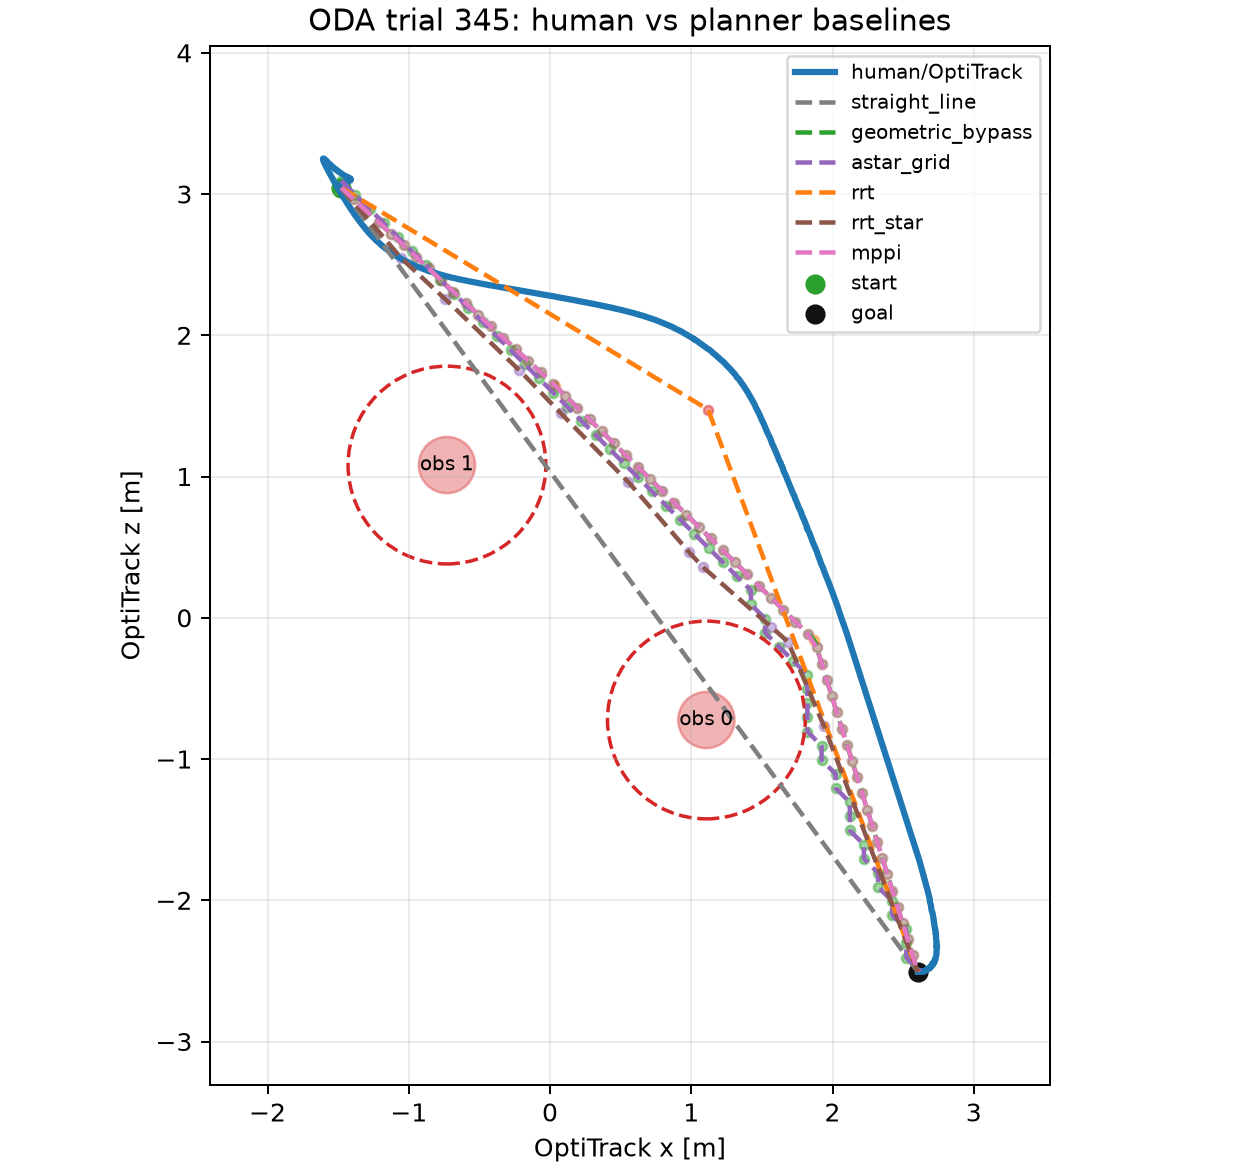
\includegraphics[width=0.82\linewidth]{planner_comparison_sample_345.png}
\caption{Ví dụ planner comparison trên trial 345.}
\end{figure}

\section{Thí nghiệm 2: Smoothness và feasibility proxy}

\textbf{Mục tiêu:} bổ sung chỉ số chất lượng quỹ đạo ngoài collision/clearance. Smoothness trong quy hoạch UAV nên được hiểu là mức độ tránh thay đổi đột ngột về hướng, vận tốc, gia tốc và lệnh điều khiển; một đường cong bo góc thường mượt hơn một đường bẻ góc, nhưng đường uốn lượn quá gắt vẫn có thể không smooth. Vì các planner ở đây chưa xuất velocity/control command, bảng chỉ báo proxy hình học 3D: path được resample theo arclength, RRT/RRT*/MPPI được bo góc bằng Chaikin smoothing nếu vẫn giữ safety clearance, rồi tính turn-angle, curvature và jerk proxy. Pose dùng frame \((x,z,y)\), trong đó \(y\) là height; planner vẫn chạy trên footprint \(x-z\) rồi lift tuyến tính lên height start--goal.

\begin{table}[H]
\centering
\small
\caption{Proxy trajectory geometry 3D trên 16 ODA local trial.}
\begin{adjustbox}{max width=\linewidth}
\begin{tabular}{lrrrrrrr}
\toprule
Method & Mean len. $\downarrow$ & P95 len. $\downarrow$ & Smooth. $\downarrow$ & P95 smooth. $\downarrow$ & Max turn $\downarrow$ & Jerk proxy $\downarrow$ & Time ms $\downarrow$ \\
\midrule
Human & 6.8853 & 8.9322 & 0.115282 & 0.418342 & 1.727 & 1135181 & 0.0 \\
RRT & 5.8320 & 7.3080 & 0.001332 & 0.008254 & 0.248 & 2099 & 1.9 \\
RRT* & 5.7257 & 7.1046 & 0.000069 & 0.000313 & 0.046 & 172 & 394.7 \\
MPPI & 5.7448 & 7.1663 & 0.000094 & 0.000384 & 0.077 & 271 & 72.0 \\
\bottomrule
\end{tabular}
\end{adjustbox}
\end{table}

\begin{figure}[H]
\centering
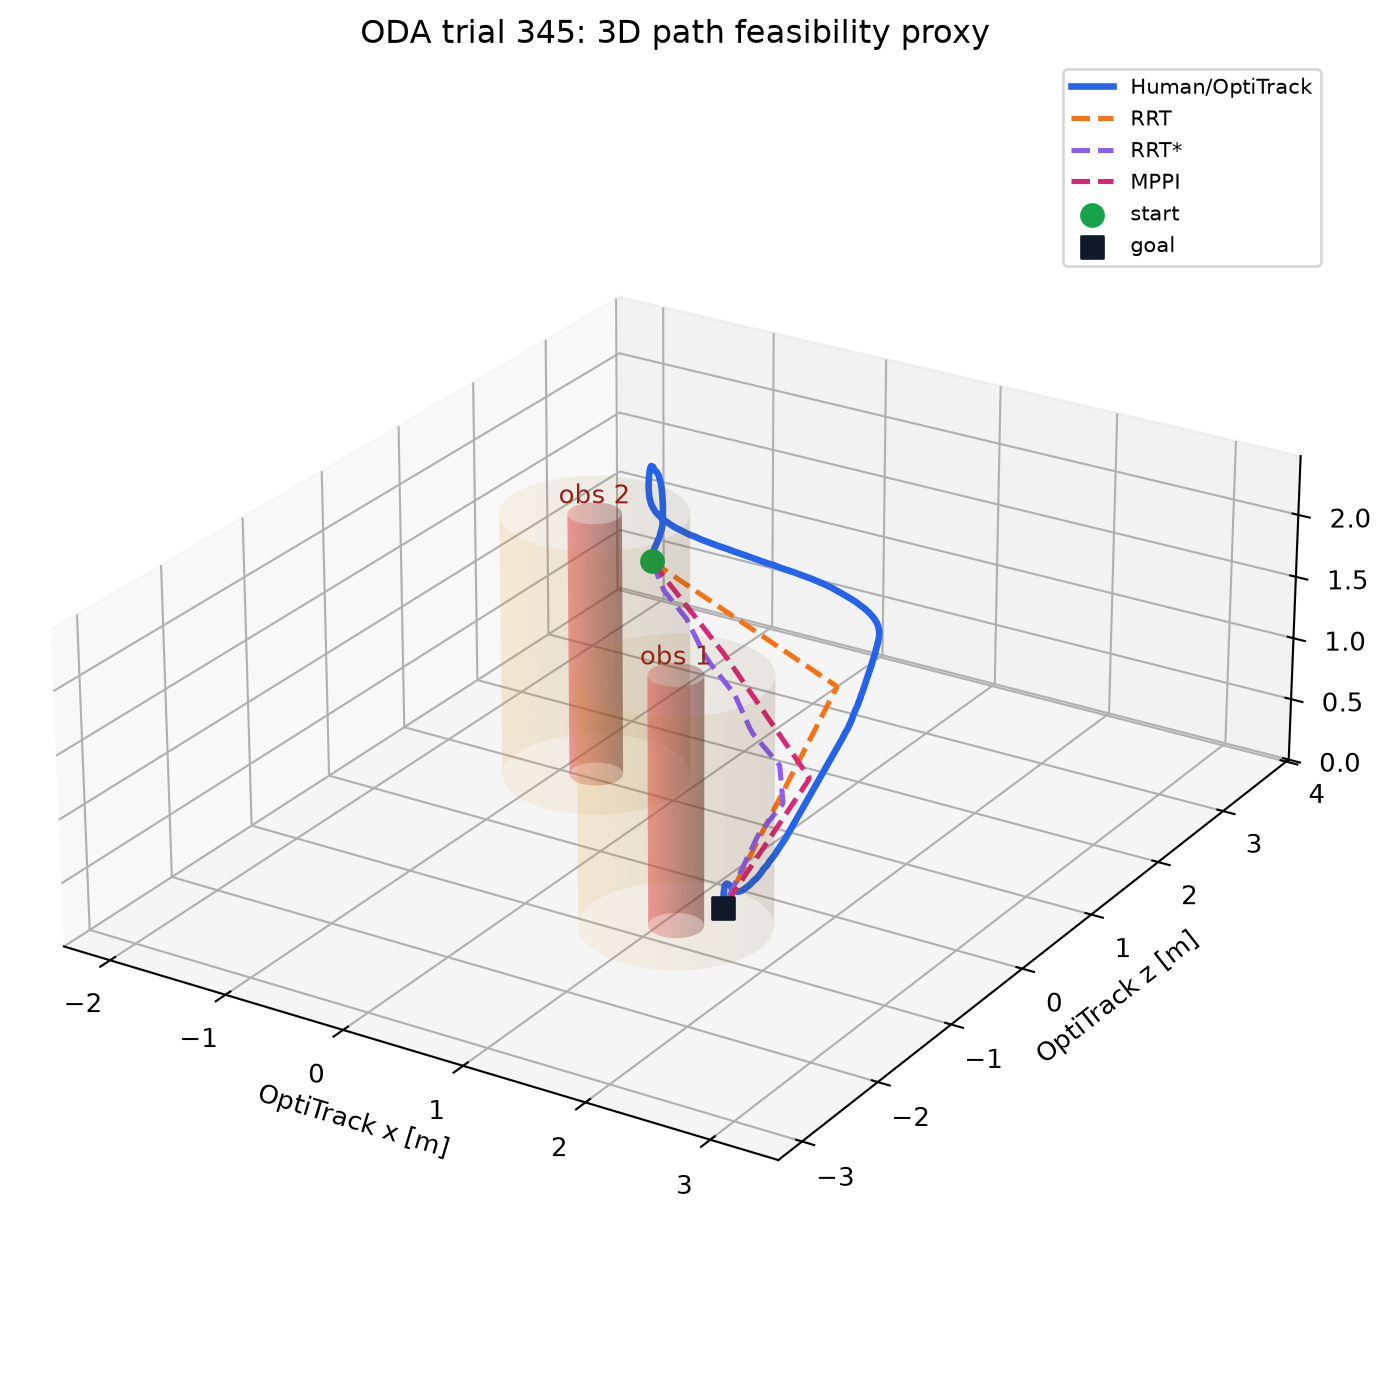
\includegraphics[width=0.78\linewidth]{trajectory_feasibility_3d_trial_345.png}
\caption{Trial 345: quỹ đạo OptiTrack 3D và path RRT/RRT*/MPPI được lift theo height để visualize proxy dynamic feasibility.}
\end{figure}

\textbf{Nhận xét:} bảng 3D này tốt hơn proxy 2D vì có tính height \(y\) của UAV và không để waypoint thưa làm góc gãy bị che mất. Sau smoothing an toàn, RRT*/MPPI có max-turn nhỏ hơn rõ rệt so với RRT. Human/OptiTrack vẫn có proxy curvature/jerk cao hơn vì quỹ đạo người lái uốn lượn và có nhiễu đo; không nên diễn giải đây là human ``kém dynamics'' nếu chưa lọc/tái tham số hóa theo thời gian. Dynamic feasibility thật cần velocity, acceleration, jerk/snap, yaw-rate, actuator/control constraints hoặc closed-loop controller log.

\section{Thí nghiệm 3: Perception-risk từ depth/radar/IMU}

\textbf{Dữ liệu:} 50 ODA trial, 2584 frame ở 5 fps. Feature gồm depth center crop, radar peak/energy/range-bin, IMU accel/gyro norm. Target là \code{future\_risk\_label}; split theo trial ID để tránh leakage.

\begin{table}[H]
\centering
\small
\caption{Future-risk classification với Depth Anything V2 Small.}
\begin{tabular}{lrrrrr}
\toprule
Feature group & Threshold & Accuracy $\uparrow$ & Macro-F1 $\uparrow$ & Bal. acc. $\uparrow$ & Risk recall $\uparrow$ \\
\midrule
Radar, macro-F1 tuned & 0.80 & 0.9053 & 0.4894 & 0.5072 & 0.0145 \\
Depth, macro-F1 tuned & 0.90 & 0.8872 & 0.4821 & 0.4972 & 0.0145 \\
Radar+IMU, macro-F1 tuned & 0.80 & 0.9025 & 0.4744 & 0.4992 & 0.0000 \\
Depth+radar+IMU, macro-F1 tuned & 0.40 & 0.9011 & 0.5918 & 0.5697 & 0.1594 \\
Radar, recall tuned & 0.05 & 0.4889 & 0.3995 & 0.5100 & 0.5362 \\
Depth, recall tuned & 0.05 & 0.7382 & 0.5504 & 0.6220 & 0.4783 \\
Radar+IMU, recall tuned & 0.05 & 0.4930 & 0.4165 & 0.5771 & 0.6812 \\
Depth+radar+IMU, recall tuned & 0.05 & 0.6602 & 0.5260 & 0.6631 & 0.6667 \\
\bottomrule
\end{tabular}
\end{table}

\textbf{Nhận xét kỹ thuật:}
\begin{itemize}
  \item Future-risk bị mất cân bằng: test positive rate khoảng 9.61\%.
  \item Accuracy cao không đủ; cần macro-F1, balanced accuracy và risk recall.
  \item Depth+radar+IMU macro-F1 tuned đạt macro-F1 0.5918, cao nhất trong bảng.
  \item Recall-tuned depth+radar+IMU đạt risk recall 0.6667 nhưng accuracy giảm xuống 0.6602.
\end{itemize}

\begin{figure}[H]
\centering
\begin{subfigure}{0.49\linewidth}
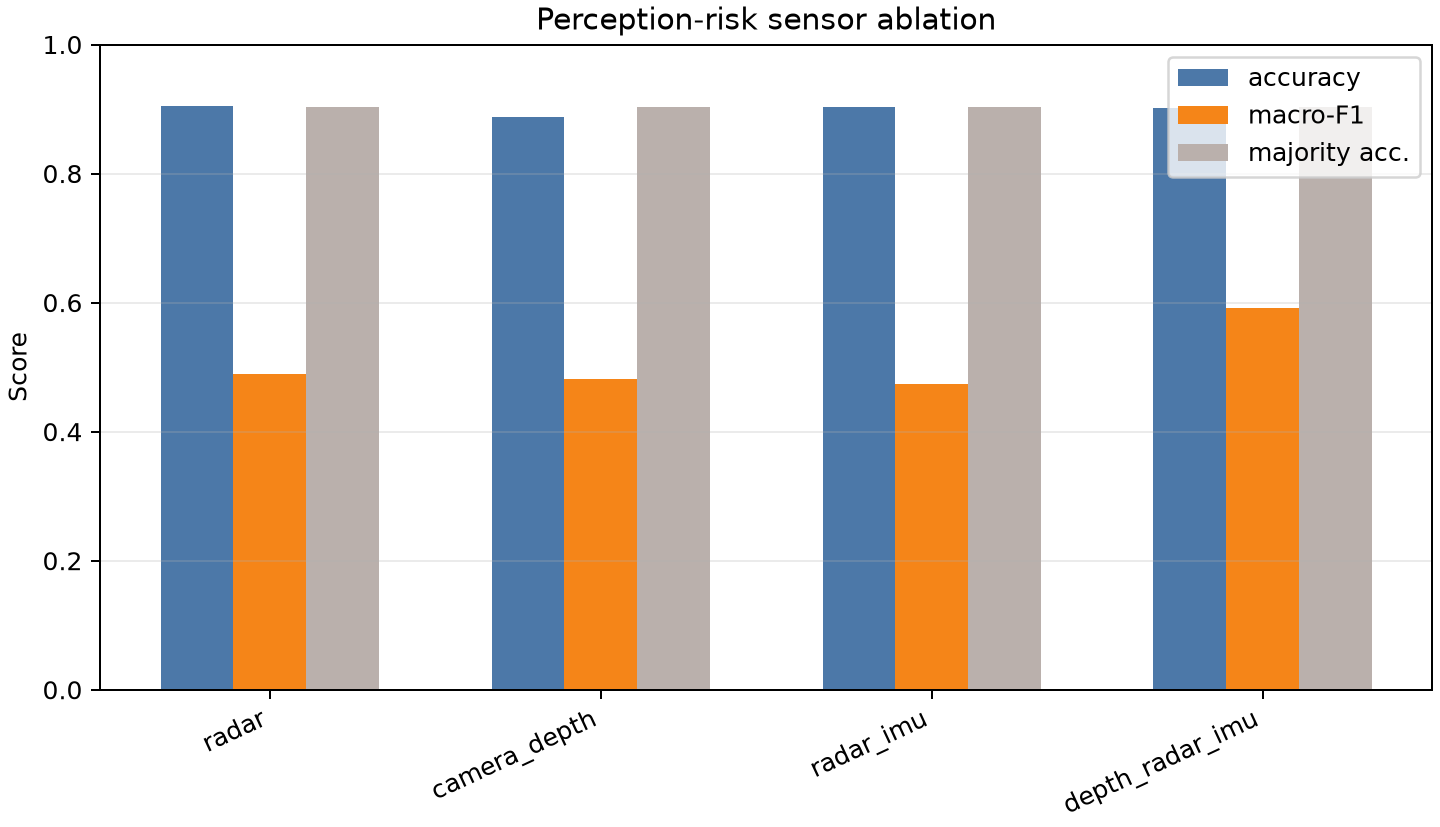
\includegraphics[width=\linewidth]{perception_risk_ablation_balanced_depth_anything_v2_small_50.png}
\caption{Macro-F1 tuned.}
\end{subfigure}
\hfill
\begin{subfigure}{0.49\linewidth}
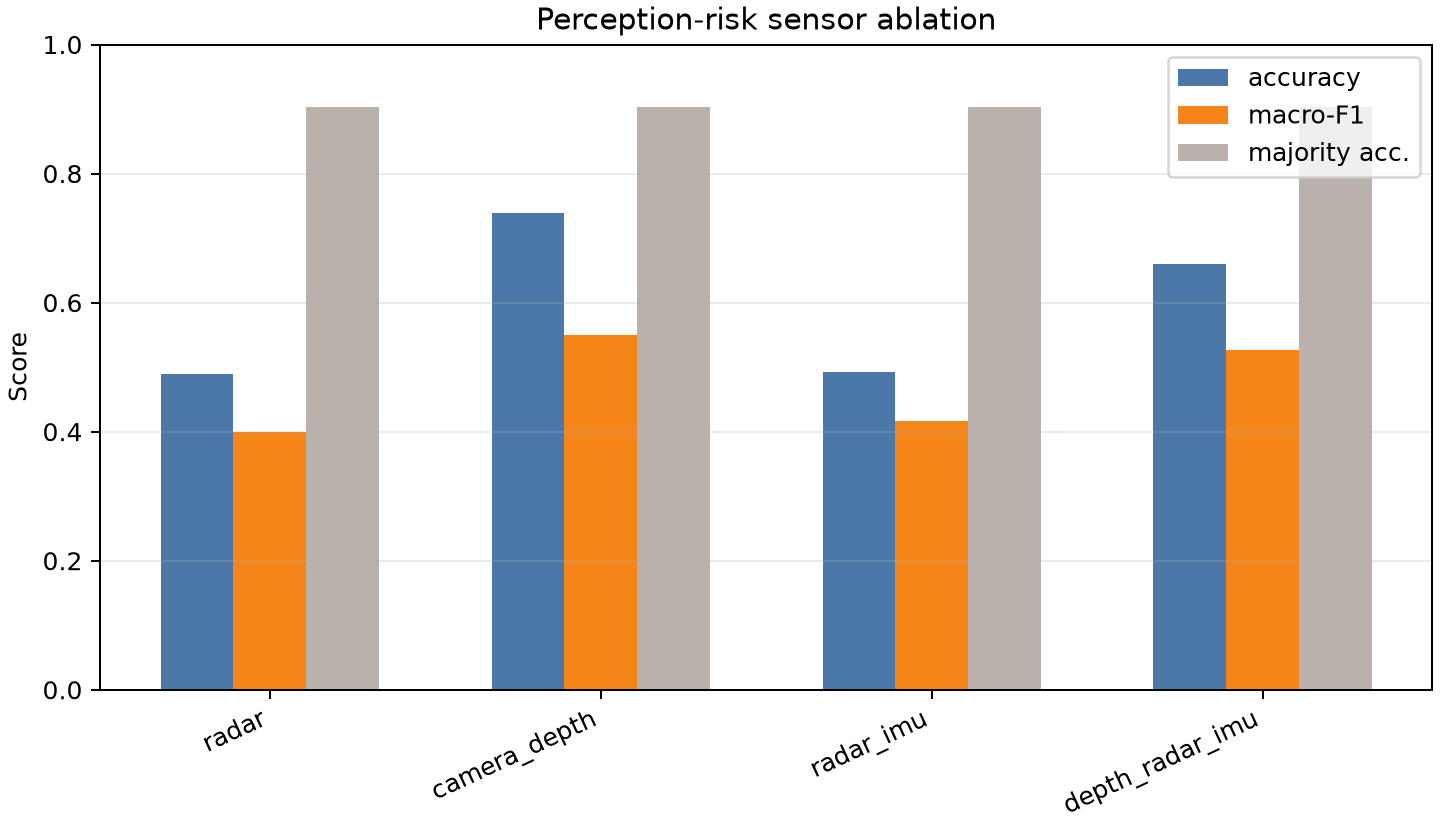
\includegraphics[width=\linewidth]{perception_risk_ablation_recall_tuned_depth_anything_v2_small_50.png}
\caption{Recall tuned.}
\end{subfigure}
\caption{Ablation perception-risk trên 50 trial.}
\end{figure}

\section{Thí nghiệm 4: Monocular depth timing và calibration}

\begin{table}[H]
\centering
\small
\caption{Depth inference timing.}
\begin{tabular}{lrrrr}
\toprule
Model/backend & Trials & Frames & Wall s/frame $\downarrow$ & Infer s/frame $\downarrow$ \\
\midrule
DPT-Hybrid/MiDaS, PyTorch & 20 & 1096 & 0.088463 & 0.042238 \\
DPT-Hybrid/MiDaS, ONNX CUDA probe & 3 & 177 & 0.082662 & 0.040498 \\
Depth Anything V2 Small, PyTorch batch & 50 & 2584 & 0.063874 & 0.017378 \\
\bottomrule
\end{tabular}
\end{table}

\begin{table}[H]
\centering
\small
\caption{Depth stability/calibration với clearance ground truth.}
\begin{tabular}{lrrrr}
\toprule
Model & Rows & Spearman $\uparrow$ & Linear RMSE m $\downarrow$ & Mean abs depth delta $\downarrow$ \\
\midrule
DPT-Hybrid/MiDaS & 1096 & 0.4752 & 1.1950 & 4.7859 \\
Depth Anything V2 Small & 2584 & 0.3251 & 1.1733 & 5.2004 \\
\bottomrule
\end{tabular}
\end{table}

\textbf{Kết luận:} depth panel dùng được cho visualization và feature tương đối, nhưng chưa đủ để claim metric depth. Cần calibration với OptiTrack/radar trước khi dùng depth làm khoảng cách theo mét.

\section{Thí nghiệm 5: Radar/IMU panel và range-Doppler}

\begin{table}[H]
\centering
\small
\caption{Radar range-Doppler summary trên sample đại diện.}
\begin{tabular}{lrrrrrr}
\toprule
Trial & Sweeps & Range bins & Mean bin & Mode bin & Zero-Doppler frac. & Entropy \\
\midrule
3 & 139 & 128 & 21.7842 & 15 & 0.1727 & 8.9222 \\
10 & 225 & 128 & 16.9644 & 3 & 0.5689 & 8.4488 \\
345 & 192 & 128 & 13.7188 & 6 & 0.5260 & 8.5293 \\
\bottomrule
\end{tabular}
\end{table}

Radar/IMU hiện dùng ở hai mức: panel định tính trong video và feature phụ cho perception-risk. Radar chưa được dùng để định vị vật cản theo mét trong benchmark chính.

\section{Thí nghiệm 6: Multi-LiDAR point-cloud segmentation}

\textbf{Mục tiêu:} đáp ứng phần LiDAR/point cloud bằng xử lý dữ liệu thật: decode point cloud, ground removal, voxel clustering, 3D axis-aligned bounding boxes. Script không yêu cầu ROS runtime.

\begin{table}[H]
\centering
\small
\caption{Point-cloud segmentation/clustering/3D bbox.}
\begin{tabular}{lrrrrr}
\toprule
Nguồn & Frames & Raw pts/frame $\uparrow*$ & FG pts/frame $\uparrow*$ & Clusters/frame $\uparrow*$ & 3D boxes $\uparrow*$ \\
\midrule
ARCO Ouster & 6 & 26324 & 9401 & 4.17 & 25 \\
Calibration Ouster & 8 & 57525 & 21403 & 3.50 & 28 \\
Calibration depth cloud & 8 & 117636 & 10422 & 1.00 & 8 \\
HolybroStdn01 Ouster & 8 & 57817 & 17594 & 8.62 & 69 \\
HolybroStdn01 Mid360 & 8 & 2004 & 1212 & 5.00 & 40 \\
HolybroStdn01 Avia & 8 & 2400 & 809 & 6.38 & 51 \\
TelloOut02 Ouster & 8 & 43209 & 6385 & 3.25 & 26 \\
TelloOut02 Mid360 & 8 & 1992 & 503 & 1.12 & 9 \\
TelloOut02 Avia & 8 & 2400 & 1748 & 1.62 & 13 \\
Tello03 Ouster & 8 & 58044 & 17530 & 7.62 & 61 \\
Tello03 Mid360 & 8 & 2004 & 1173 & 5.38 & 43 \\
Tello03 Avia & 8 & 2400 & 1042 & 5.62 & 45 \\
\bottomrule
\end{tabular}
\end{table}

\begin{figure}[H]
\centering
\includegraphics[width=0.94\linewidth]{multilidar_tello03_ouster_pointcloud_3d_bboxes.png}
\caption{Tello03 Ouster: voxel clusters và 3D AABB.}
\end{figure}

\textbf{Nhận xét kỹ thuật:}
\begin{itemize}
  \item Tello03 tạo 149 bbox 3D trên 24 sensor-frame; TelloOut02 tạo 48 bbox 3D; HolybroStdn01 tạo 160 bbox 3D.
  \item Ouster có mật độ điểm cao hơn Livox trong các frame mẫu.
  \item Multi-LiDAR dùng để kiểm tra sensing/generalization; không dùng để tính collision metric UAV của ODA.
\end{itemize}

\section{Thí nghiệm 7: Lightweight 3D simulation}

\textbf{Mục tiêu:} tạo demo 3D có thể mở ngay trên laptop để minh họa pipeline từ biểu diễn vật cản sang obstacle map và đường bay planner. Demo dùng Three.js, không phụ thuộc ROS/Gazebo runtime.

\begin{figure}[H]
\centering
\includegraphics[width=0.96\linewidth]{uav_3d_sim_desktop.png}
\caption{3D simulation: obstacle/safety volume, occupancy footprint, 3D bbox, planner path và UAV marker.}
\end{figure}

\begin{table}[H]
\centering
\small
\caption{Kết quả planner trong scene 3D demo.}
\begin{tabular}{lrrrr}
\toprule
Planner & Waypoints & Path length (m) $\downarrow$ & Min clearance (m) $\uparrow$ & Safety violation $\downarrow$ \\
\midrule
RRT & 14 & 7.1828 & 0.7017 & No \\
MPPI & 60 & 6.6809 & 0.6191 & No \\
\bottomrule
\end{tabular}
\end{table}

Verifier bằng Chrome headless đã tạo screenshot desktop/mobile và kiểm tra pixel WebGL không rỗng. Đây là visual simulation để trình bày quá trình \(\text{obstacle geometry} \rightarrow \text{occupancy/safety map} \rightarrow \text{planner path} \rightarrow \text{UAV motion}\). Demo chưa claim physics-level quadrotor dynamics; Gazebo/ROS2 vẫn là bước runtime simulation thật.

\section{Thí nghiệm 8: ROS2/Gazebo fused costmap và 3D fused POV}

\textbf{Mục tiêu:} bổ sung minh chứng runtime rằng output perception có thể được đưa vào planner dưới dạng costmap, thay vì chỉ dừng ở visualization offline. Nhánh này không thay thế benchmark ODA chính; nó kiểm chứng hợp đồng dữ liệu \(\text{sensor/perception} \rightarrow \text{OccupancyGrid} \rightarrow \text{planner path}\).

\begin{table}[H]
\centering
\small
\caption{Runtime evidence cho mode fused ROS2/Gazebo.}
\begin{tabularx}{0.98\linewidth}{>{\bfseries}p{3.6cm} X}
\toprule
Hạng mục & Kết quả \\
\midrule
Mode kiểm chứng & \code{gazebo\_fused} fused-costmap runtime. \\
Sensor/source input & Synthetic PointCloud2, Gazebo depth image và Gazebo LaserScan. \\
Source costmap & \code{/perception/pointcloud\_occupancy\_grid}, \code{/perception/depth\_occupancy\_grid}, \code{/perception/laserscan\_occupancy\_grid}. \\
Fused output & \code{costmap\_mux} merge thành \code{/perception/occupancy\_grid}; planner publish \code{/planned\_path}. \\
Verifier & 13/13 required topics present, 13/13 message samples received, mux status \code{passed}. \\
Evidence & Runtime log trong \code{outputs/ros2\_demo\_runtime/}; video fused-sensor runtime trong \code{outputs/videos/}. \\
\bottomrule
\end{tabularx}
\end{table}

\textbf{Offline contract kiểm tra lại ngày 01/07/2026:} để tránh chỉ dựa vào mô tả ROS2, report bổ sung một kiểm tra không cần ROS runtime. Script đọc output perception hoặc depth proxy, chuyển về occupancy grid, rồi gọi cùng planner helper. Năm nguồn perception đều sinh map không rỗng và path hợp lệ; matrix planner local kiểm tra RRT và MPPI đều collision-free sau inflation.

\begin{table}[H]
\centering
\small
\caption{Perception-to-planner contract và matrix planner local.}
\begin{tabularx}{0.98\linewidth}{>{\bfseries}p{4.0cm} r r X}
\toprule
Nguồn perception & Grid & Occupied & Kết quả planner \\
\midrule
LiDAR bbox CSV & \(88 \times 72\) & 626 & RRT/MPPI đều collision-free. \\
Metric depth image & \(80 \times 80\) & 269 & RRT/MPPI đều collision-free. \\
Relative predicted-depth proxy & \(80 \times 80\) & 30 & RRT/MPPI đều collision-free. \\
LiDAR bbox + relative-depth mux & \(133 \times 75\) & 638 & RRT/MPPI đều collision-free. \\
LiDAR bbox + cached-depth mux & \(133 \times 75\) & 666 & RRT/MPPI đều collision-free. \\
\bottomrule
\end{tabularx}
\end{table}

Sau khi có runtime evidence, demo 3D được cập nhật để thể hiện rõ sensor fusion trong không gian 3D: cyan là point-cloud evidence, đỏ/cam là LiDAR scan/grid, tím là depth evidence/grid, xanh lá là fused occupancy grid mà planner dùng. Bản POV của drone có thêm inset góc dưới phải: heatmap relative depth và fan-scan LiDAR theo thời gian thực.

\begin{figure}[H]
\centering
\includegraphics[width=0.96\linewidth]{uav_3d_fused_sensor_pov_inset_preview.png}
\caption{POV từ drone trong demo 3D fused: cảnh chính hiển thị obstacle, point cloud, depth evidence và fused grid; inset góc dưới phải hiển thị relative depth map và LiDAR scan input tại cùng thời điểm bay.}
\end{figure}

\begin{figure}[H]
\centering
\includegraphics[width=0.98\linewidth]{uav_3d_fused_sensor_multiview_preview.png}
\caption{Video multiview fused 3D: cột trái là external 3D, cột giữa là drone POV với depth/LiDAR inset, cột phải là top-down view của fused grid và planner path.}
\end{figure}

\textbf{Kết luận kỹ thuật:} hiện đã có hai lớp minh chứng bổ sung cho báo cáo tiến độ: (i) ROS2/Gazebo verifier chứng minh costmap fusion chạy được ở runtime và planner nhận được fused occupancy grid; (ii) WebGL 3D multiview giúp trình bày trực quan quá trình drone bay, cảm biến nhìn thấy vật cản và fused grid được hình thành. Giới hạn vẫn là fixed-altitude 2D planning; PX4/offboard chưa được claim là đã verify runtime trên server này.

\section{Thí nghiệm 9: Full 3D voxel/ESDF và MPPI}

\textbf{Mục tiêu:} nâng nhánh simulation từ occupancy grid 2D/fixed-altitude sang biểu diễn gần robot thật hơn: voxel occupancy 3D, Euclidean Signed Distance Field (ESDF), và MPPI tối ưu quỹ đạo liên tục trong không gian \(x,y,z\). Đây là bước trung gian trước khi thay map synthetic bằng ESDF/voxel map sinh online từ depth hoặc LiDAR.

\begin{table}[H]
\centering
\small
\caption{Kết quả demo 3D ESDF/MPPI trong môi trường indoor synthetic.}
\begin{tabularx}{0.86\linewidth}{>{\bfseries}p{4.0cm} X}
\toprule
Chỉ số & Giá trị \\
\midrule
Map resolution & \(0.15\,m\) \\
Occupied voxels & 3084 / 43680 \\
MPPI horizon / rollouts / iterations & 72 / 768 / 12 \\
Path length $\downarrow$ & \(7.6455\,m\) \\
Altitude change $\downarrow$ & \(0.4499\,m\) \\
Minimum ESDF distance $\uparrow$ & \(0.6783\,m\) \\
Minimum safety margin $\uparrow$ & \(0.2583\,m\) \\
Collision / safety violation $\downarrow$ & 0 / 0 \\
Local compute time $\downarrow$ & \(123.638\,ms\) \\
Server compute time, RTX 2060 SUPER $\downarrow$ & \(357.047\,ms\) \\
Cost reduction vs. direct line $\uparrow$ & \(99.86\%\) \\
\bottomrule
\end{tabularx}
\end{table}

\begin{figure}[H]
\centering
\includegraphics[width=0.96\linewidth]{indoor_3d_esdf_mppi_path.png}
\caption{Full 3D ESDF/MPPI: path đổi cao độ để tránh vật cản trong voxel map; subplot phải là ESDF slice dùng để kiểm tra vùng clearance.}
\end{figure}

\textbf{Ý nghĩa kỹ thuật:} planner không còn kiểm tra ô occupied/free nhị phân. Mỗi rollout MPPI query khoảng cách tới vật cản:
\[
d = \mathrm{ESDF}(x,y,z),\qquad
J_{\mathrm{clearance}} = w_c \max(0, r_{\mathrm{safe}}-d)^2.
\]
Cách này phù hợp hơn với UAV indoor vì trajectory có thể đổi cao độ và cost thay đổi mượt theo khoảng cách tới vật cản.

\textbf{Trạng thái NVBlox trên server:} server ROS2 Jazzy + GPU đã cài thành công Isaac ROS/NVBlox. Readiness check detect được \code{nvblox\_ros}, \code{nvblox\_msgs}, \code{isaac\_ros\_nvblox}, \code{ros\_gz\_bridge}, \code{rviz2}; các executable gồm \code{nvblox\_node}, \code{fuser\_node}, \code{fuse\_cusfm}. Package ROS2 của project build được và publish replay \code{/planned\_path\_3d}, \code{/esdf3d\_mppi\_markers}. Server đã chạy được ba nhánh vào NVBlox: synthetic depth, Gazebo depth và organized \code{PointCloud2} LiDAR. Bước mới nhất verify \code{PointCloud2} LiDAR \(\rightarrow\) planner-side local 3D ESDF \(\rightarrow\) MPPI trong khi NVBlox đang chạy \code{esdf\_mode=3d} và publish \code{/nvblox\_node/tsdf\_layer}.

\begin{table}[H]
\centering
\small
\caption{Smoke test NVBlox DistanceMapSlice \(\rightarrow\) MPPI planner.}
\begin{tabularx}{0.99\linewidth}{>{\bfseries}p{2.7cm} >{\raggedright\arraybackslash}X >{\raggedright\arraybackslash}X >{\raggedright\arraybackslash}X}
\toprule
Chỉ số & Synthetic depth & Gazebo depth & PointCloud2 LiDAR \\
\midrule
Sensor input & Depth image + CameraInfo & Gazebo depth image & Organized \code{PointCloud2}, \(360 \times 16\) beams \\
DistanceMapSlice & \(105 \times 160\), \(0.05\,m\) & \(105 \times 160\), \(0.05\,m\) & \(169 \times 288\), \(0.05\,m\) \\
Slice height & \(1.20\,m\) & \(1.20\,m\) & \(1.20\,m\) \\
Planner & MPPI over NVBlox slice & MPPI over NVBlox slice & MPPI over NVBlox slice \\
Waypoints & 56 & 56 & 56 \\
Minimum distance $\uparrow$ & \(0.45\,m\) & \(2.00\,m\) & \(2.00\,m\) \\
Safety violation $\downarrow$ & False & False & False \\
Compute time $\downarrow$ & \(215.572\,ms\) & \(272.500\,ms\) & \(239.518\,ms\) \\
NVBlox sensor / ESDF rate $\uparrow$ & \(10.1 / 4.9\,Hz\) & \(9.4 / 4.9\,Hz\) & \(10.1 / 4.9\,Hz\) \\
\bottomrule
\end{tabularx}
\end{table}

\begin{table}[H]
\centering
\small
\caption{Verifier mới: PointCloud2 LiDAR \(\rightarrow\) local 3D ESDF \(\rightarrow\) MPPI, chạy song song với NVBlox 3D TSDF runtime.}
\begin{tabularx}{0.92\linewidth}{>{\bfseries}p{4.0cm} X}
\toprule
Chỉ số & Giá trị \\
\midrule
Sensor input & Organized \code{PointCloud2}, \(360 \times 24\) beams \\
NVBlox runtime & \code{esdf\_mode=3d}, \code{/nvblox\_node/tsdf\_layer} type \code{nvblox\_msgs/msg/VoxelBlockLayer} \\
Planner map & Local 3D occupancy ESDF từ PointCloud2, resolution \(0.12\,m\) \\
ESDF grid & \(43 \times 33 \times 29\) voxels; z-span \(3.36\,m\); known voxels 41151 \\
Planner & MPPI \(x,y,z\), 52 waypoints \\
Minimum ESDF distance $\uparrow$ & \(0.5648\,m\) \\
Safety radius / violation $\downarrow$ & \(0.45\,m\) / False \\
Path length / altitude change $\downarrow$ & \(2.9033\,m\) / \(0.2499\,m\) \\
Planner compute time $\downarrow$ & \(18.433\,ms\) \\
NVBlox sensor / ESDF rate $\uparrow$ & LiDAR \(\approx 10.1\,Hz\), ESDF update \(\approx 4.9\,Hz\) \\
\bottomrule
\end{tabularx}
\end{table}

\textbf{Giới hạn còn lại:} nhánh full 3D mới dùng ESDF local do planner tạo từ \code{PointCloud2}; NVBlox được verify ở mức 3D TSDF/ESDF runtime song song nhưng chưa export/query trực tiếp toàn bộ 3D ESDF volume trong planner. Hệ thống cũng chưa closed-loop UAV control bằng setpoint động; đây là bước tiếp theo nếu chuyển sang PX4/offboard hoặc Gazebo controller.

\section{Thí nghiệm 10: Online latency và kinematic feasibility proxy 10 Hz}

\textbf{Mục tiêu:} trả lời trực tiếp câu hỏi mentor về khả năng chạy online, thay vì nhảy ngay sang full AvoidBench. Thí nghiệm giả lập pipeline hẹp:
\[
\text{LiDAR 3D }10\,Hz \rightarrow \text{occupancy/ESDF update} \rightarrow \text{MPPI }x,y,z \rightarrow \text{command}.
\]
Latency được tính theo worst-case sensor period:
\[
T_{\mathrm{delay}} = 100\,ms + T_{\mathrm{map}} + T_{\mathrm{MPPI}} + 10\,ms,
\qquad
d_{\mathrm{delay}} = v_{\mathrm{UAV}}T_{\mathrm{delay}}.
\]
Trong thời gian delay, UAV tiếp tục bay thẳng theo command cũ; MPPI sau đó replan từ pose đã bị trễ. Body radius dùng để báo collision là \(0.20\,m\), safety radius của MPPI là \(0.45\,m\). Đây là kinematic delay check trên scene ESDF 3D synthetic, chưa phải full quadrotor dynamics/PX4 closed-loop.

\begin{table}[H]
\centering
\small
\caption{Online latency kinematic proxy: LiDAR 3D 10 Hz \(\rightarrow\) ESDF \(\rightarrow\) MPPI.}
\begin{tabular}{rrrrrrrrr}
\toprule
Sensor Hz & Speed & Map ms $\downarrow$ & MPPI ms $\downarrow$ & Total ms $\downarrow$ & Delay m $\downarrow$ & Min clr. $\uparrow$ & Coll. $\downarrow$ & Viol. $\downarrow$ \\
\midrule
10 & 1.0 & 5.9 & 28.9 & 144.7 & 0.145 & 0.389 & 0 & 0 \\
10 & 2.0 & 5.9 & 87.4 & 203.3 & 0.407 & 0.268 & 0 & 0 \\
10 & 3.0 & 5.9 & 187.8 & 303.7 & 0.911 & 0.523 & 0 & 0 \\
10 & 4.0 & 5.9 & 184.5 & 300.3 & 1.201 & 0.403 & 0 & 0 \\
10 & 5.0 & 5.9 & 205.5 & 321.4 & 1.607 & 0.125 & 0 & 1 \\
10 & 6.0 & 5.9 & 184.6 & 300.4 & 1.803 & -0.015 & 1 & 1 \\
\bottomrule
\end{tabular}
\end{table}

\begin{figure}[H]
\centering
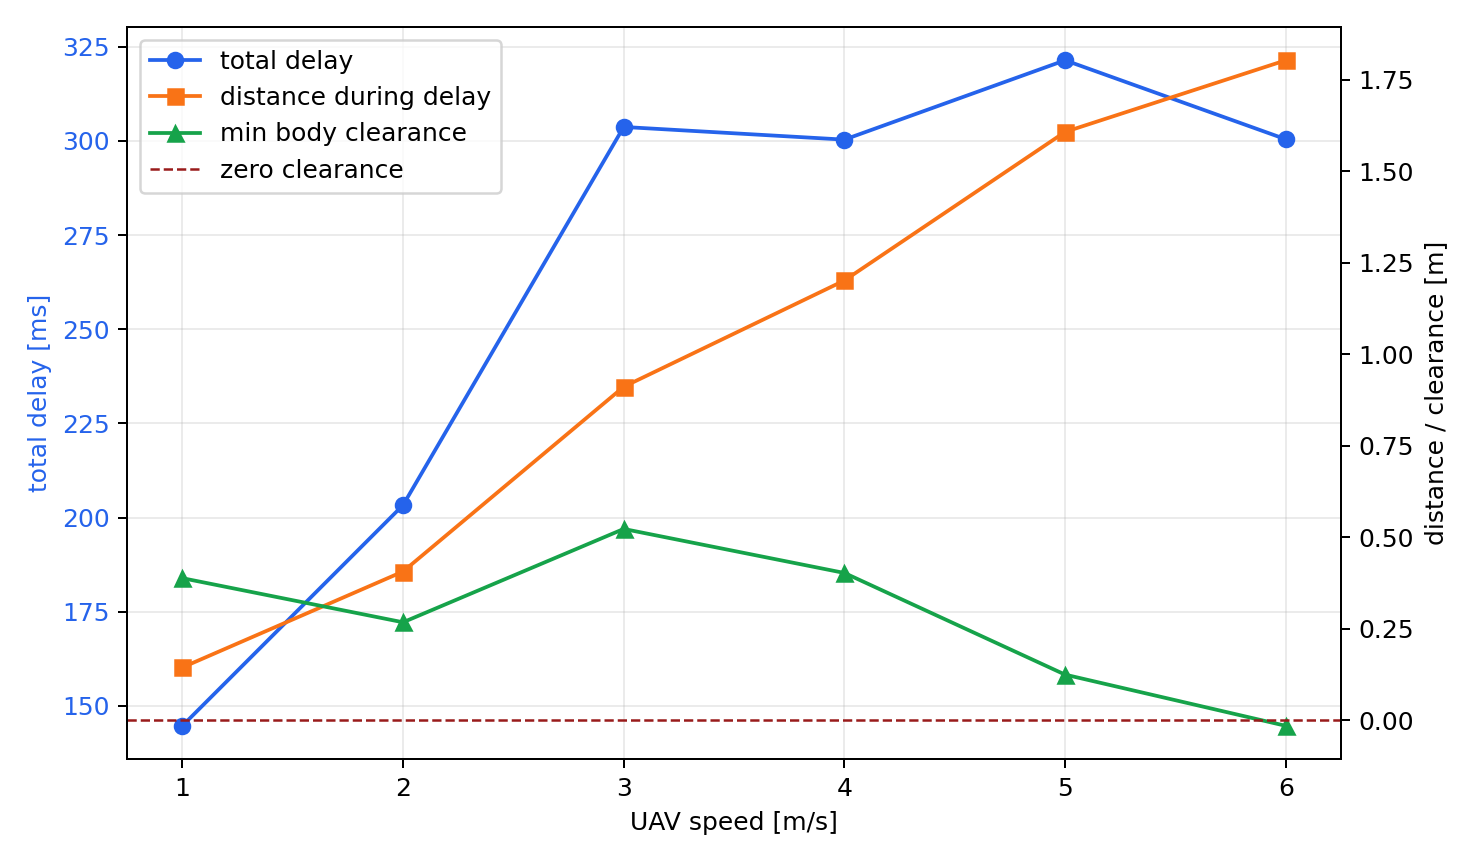
\includegraphics[width=0.84\linewidth]{online_latency_feasibility_10hz.png}
\caption{Tổng delay, quãng đường UAV đi trong delay, và minimum body-clearance sau khi replan.}
\end{figure}

\textbf{So sánh thêm với planner baseline ở cùng online 10 Hz:} để kiểm tra không chỉ riêng MPPI, report chạy thêm \(3\) planner \(\times\) \(6\) tốc độ \(\times\) \(8\) case \(=144\) case. RRT, RRT* và MPPI dùng seeded sampling. RRT/RRT* là baseline 2D fixed-altitude ở \(z=1.50\,m\), sau đó lift path lên 3D ESDF để chấm clearance; MPPI là planner 3D ESDF. Failure của planner được tính vào nhóm collision/unsafe vì UAV không có command tránh vật cản hợp lệ.

\begin{table}[H]
\centering
\scriptsize
\caption{Online 10 Hz planner rate qua 8 synthetic kinematic-latency case mỗi tốc độ. Mỗi ô có dạng Safe/Viol./Coll. \%.}
\begin{tabularx}{0.98\linewidth}{>{\bfseries}p{2.6cm} c c c c c c}
\toprule
Planner & 1 m/s & 2 m/s & 3 m/s & 4 m/s & 5 m/s & 6 m/s \\
\midrule
RRT & 62.5/37.5/0 & 62.5/37.5/0 & 75/25/0 & 50/50/0 & 75/25/0 & 87.5/12.5/0 \\
RRT* & 87.5/12.5/0 & 75/25/0 & 37.5/62.5/0 & 50/50/0 & 62.5/25/12.5 & 0/12.5/87.5 \\
MPPI 3D ESDF & 100/0/0 & 100/0/0 & 100/0/0 & 100/0/0 & 0/37.5/62.5 & 0/75/25 \\
\bottomrule
\end{tabularx}
\end{table}

\textbf{Timing trung bình của planner comparison:} RRT \(2.8\,ms\) compute / \(118.7\,ms\) total delay; RRT* \(98.8\,ms\) / \(214.7\,ms\); MPPI 3D ESDF \(161.5\,ms\) / \(277.4\,ms\). MPPI 3D giữ \(100\%\) safe tới \(4\,m/s\) trong proxy synthetic này, nhưng ở \(5\,m/s\) bắt đầu unsafe do tổng delay lớn hơn. RRT/RRT* có compute nhanh hơn MPPI nhưng stochastic path clearance dao động, nên có safety violation ngay cả ở tốc độ thấp trong một số seed.

\textbf{Nhận xét kỹ thuật:}
\begin{itemize}
  \item Ở \(2\,m/s\), tổng delay đo được khoảng \(203\,ms\), nên UAV đi thêm \(0.41\,m\) trước khi command mới có hiệu lực. Case này chỉ còn safety margin khoảng \(0.018\,m\), nghĩa là rất sát ngưỡng an toàn dù chưa collision.
  \item Ở \(5\,m/s\), UAV đi khoảng \(1.61\,m\) trong delay và đã vào vùng safety radius: safety violation = 1 dù body-clearance vẫn còn \(0.125\,m\).
  \item Ở \(6\,m/s\), UAV đi khoảng \(1.80\,m\) trong delay; body-clearance xuống \(-0.015\,m\), tức là collision trong kiểm tra kinematic-delay này.
  \item Kết quả này trả lời phần online timing ở mức proxy: pipeline cần được đánh giá bằng latency và khoảng cách UAV đi trong delay, nhưng chưa thay cho mô phỏng dynamics vật lý đầy đủ. Nếu vật cản xuất hiện ở tầm \(0.5\)--\(1.0\,m\), cấu hình hiện tại sẽ rất căng; nếu có \(3\)--\(5\,m\) lookahead thì còn khả thi hơn.
\end{itemize}

\textbf{ODA replay 3D với cấu hình giả lập Jetson:} report bổ sung một biến thể bám sát ODA hơn. Với 16 trial local \((1\)--\(15,345)\), mỗi trial chọn 8 timestamp gần obstacle nhất theo clearance 3D. Tại mỗi timestamp \(t\), pipeline dùng pose ODA \(p(t)=(x,z,y)\), tạo local voxel/costmap từ obstacle cylinder trong \code{trial\_overview.csv}. Bản này dùng profile giả lập Jetson Orin Nano-class gồm sensor 10 Hz, \(20\,ms\) pipeline I/O, costmap/planner được scale từ timing Python local, và \(15\,ms\) command overhead. Đây là profile onboard đại diện để báo cáo timing tổng, chưa phải benchmark thật trên Jetson. RRT, RRT* và MPPI vẫn sinh path trên footprint \(x-z\), sau đó path được lift tuyến tính theo height để tính clearance 3D tới finite cylinder obstacle. Vận tốc báo cáo là displacement speed 3D trong cửa sổ \(0.25\,s\) quanh timestamp.

\begin{table}[H]
\centering
\small
\caption{ODA replay feasibility 3D với profile giả lập Jetson: 16 trial \(\times\) 8 timestamp gần obstacle \(\times\) 3 planner \(=384\) case.}
\begin{tabular}{lrrrrrr}
\toprule
Planner & Cases & Safe \% $\uparrow$ & Viol. \% $\downarrow$ & Coll. \% $\downarrow$ & Total ms $\downarrow$ & Planner ms $\downarrow$ \\
\midrule
RRT & 128 & 89.8 & 0.8 & 9.4 & 149.9 & 11.2 \\
RRT* & 128 & 88.3 & 0.8 & 10.9 & 181.6 & 42.9 \\
MPPI & 128 & 88.3 & 11.7 & 0.0 & 169.7 & 31.0 \\
\bottomrule
\end{tabular}
\end{table}

\textbf{Ý nghĩa của ODA replay 3D:} MPPI không collision nhưng có safety violation \(11.7\%\); RRT/RRT* có một số planner failure trong các timestamp gần obstacle, được tính vào nhóm collision/unsafe vì không tạo được command tránh vật cản hợp lệ. Giá trị chính của bảng là kiểm tra được metric 3D trên OptiTrack \((x,z,y)\), dùng obstacle cylinder hữu hạn từ metadata ODA, và báo cáo timing tổng dưới một profile onboard đại diện. Không dùng bảng này để claim runtime thật trên Jetson hoặc kết luận operating envelope closed-loop.

\section{Thí nghiệm 11: Sensor-to-occupancy latency}

\textbf{Mục tiêu:} thay giả định ideal occupancy ở thí nghiệm 10 bằng thời gian xử lý của các frontend hiện có trong project. Đây vẫn là replay/offline compute latency, không phải driver/hardware latency thật. Với ODA, chỉ RGB/depth/radar/IMU có dữ liệu; radar/IMU hiện chỉ tạo feature/risk, chưa tạo occupancy grid nên không đưa vào bảng này. LiDAR dùng hàng \code{Multi-LiDAR bbox} là external stress-test, không phải ODA.

\begin{table}[H]
\centering
\small
\caption{Sensor frontend \(\rightarrow\) occupancy grid \(\rightarrow\) MPPI: ngưỡng đáp ứng theo tốc độ UAV.}
\begin{tabularx}{0.98\linewidth}{>{\bfseries}p{3.5cm} r r r r r r}
\toprule
Frontend & Sensor ms $\downarrow$ & Frontend ms $\downarrow$ & Delay@2m/s $\downarrow$ & Max safe $\uparrow$ & First viol. $\uparrow$ & First coll. $\uparrow$ \\
\midrule
Ideal occupancy/ESDF & 100.0 & 5.9 & 200.7 & 4.0 & 5.0 & 6.0 \\
ODA cached depth-to-grid & 200.0 & 2.3 & 300.4 & 3.0 & 4.0 & 5.0 \\
ODA Depth Anything-to-grid & 200.0 & 66.2 & 364.2 & 2.0 & 3.0 & 4.0 \\
External LiDAR bbox-to-grid & 100.0 & 0.02 & 201.2 & 4.0 & 5.0 & \(>6.0\) \\
BBox + cached depth mux & 200.0 & 2.7 & 299.9 & 3.0 & 4.0 & 5.0 \\
\bottomrule
\end{tabularx}
\end{table}

\begin{figure}[H]
\centering
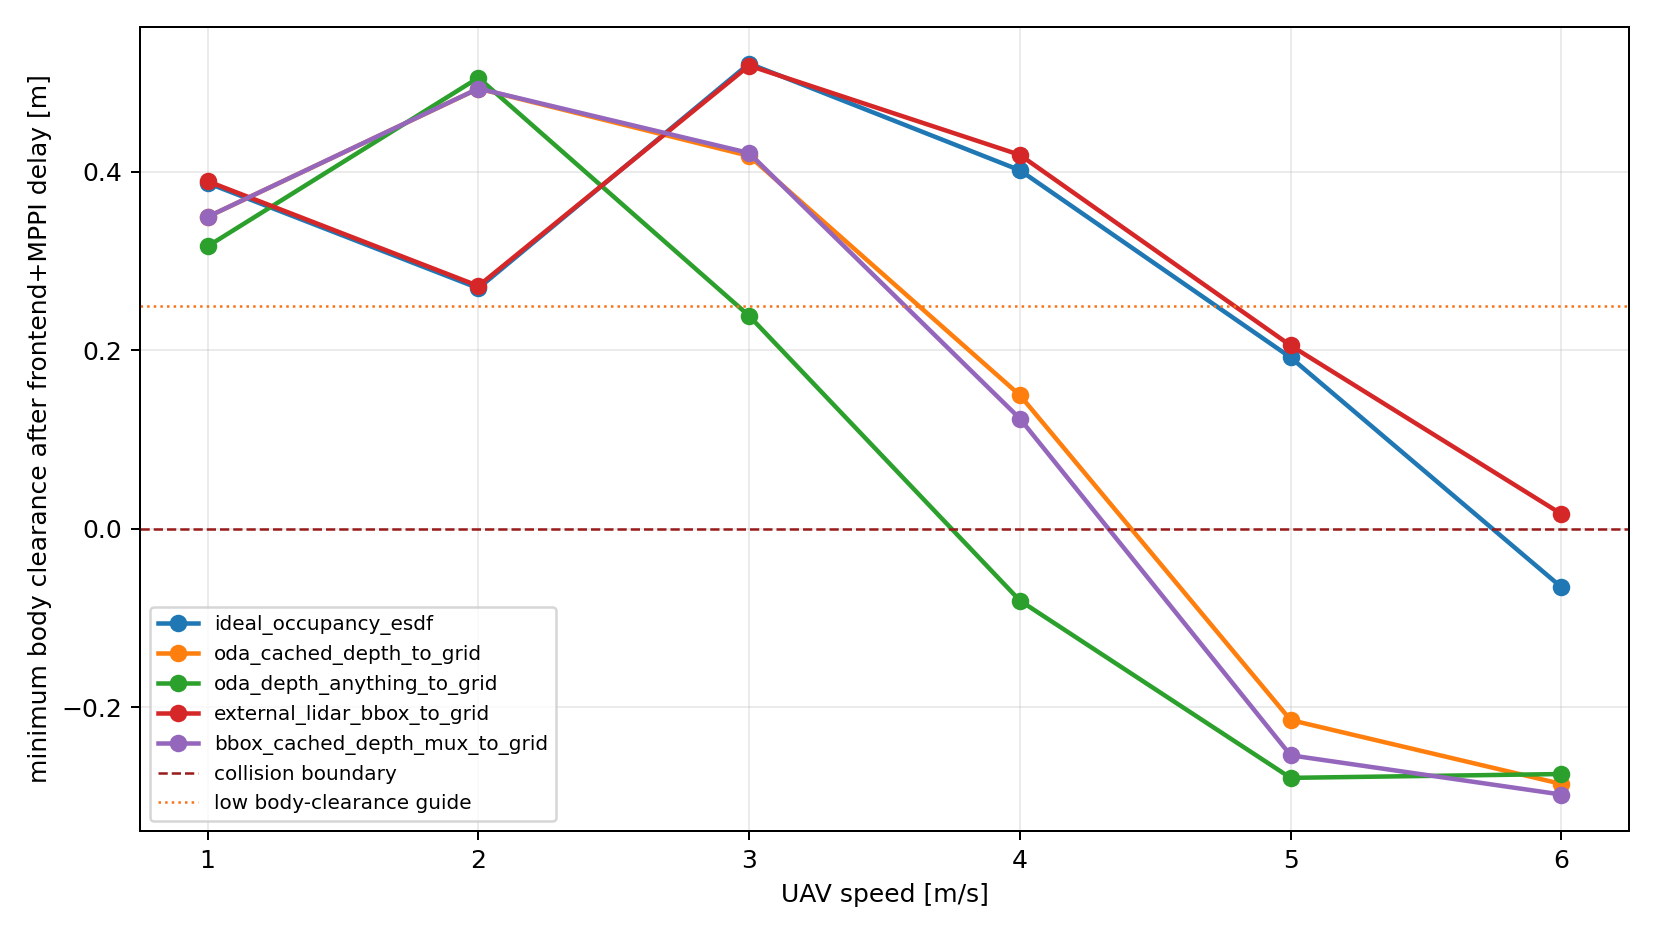
\includegraphics[width=0.86\linewidth]{sensor_frontend_latency_feasibility.png}
\caption{Minimum body-clearance khi cộng thêm latency của từng frontend sensor-to-occupancy trước MPPI.}
\end{figure}

\begin{table}[H]
\centering
\scriptsize
\caption{Tỷ lệ safe/violation/collision qua 8 MPPI seed cho mỗi tốc độ. Mỗi ô có dạng Safe/Viol./Coll. \%.}
\begin{tabularx}{0.98\linewidth}{>{\bfseries}p{3.4cm} c c c c c}
\toprule
Frontend & 2 m/s & 3 m/s & 4 m/s & 5 m/s & 6 m/s \\
\midrule
Ideal occupancy/ESDF & 100/0/0 & 87.5/12.5/0 & 62.5/12.5/25 & 0/100/0 & 0/0/100 \\
ODA cached depth-to-grid & 100/0/0 & 100/0/0 & 0/87.5/12.5 & 0/0/100 & 0/0/100 \\
ODA Depth Anything-to-grid & 100/0/0 & 62.5/37.5/0 & 0/0/100 & 0/0/100 & 0/0/100 \\
External LiDAR bbox-to-grid & 100/0/0 & 100/0/0 & 100/0/0 & 0/100/0 & 0/0/100 \\
BBox + cached depth mux & 100/0/0 & 87.5/12.5/0 & 0/87.5/12.5 & 0/0/100 & 0/0/100 \\
\bottomrule
\end{tabularx}
\end{table}

\textbf{Nhận xét kỹ thuật:}
\begin{itemize}
  \item Bảng tỷ lệ dùng 8 seed MPPI cho mỗi cặp frontend/tốc độ, tổng cộng 240 case. \code{Violation} là safety-radius violation nhưng chưa body collision; \code{collision} được đếm riêng.
  \item Với ODA cached depth, bản thân bước projection depth-to-grid rất nhanh, khoảng \(2.3\,ms\). Bottleneck chính là sensor/update period \(5\,fps \Rightarrow 200\,ms\), nên max safe speed trong check này giảm còn khoảng \(3\,m/s\).
  \item Khi tính cả Depth Anything V2 Small replay wall-time, frontend tăng lên khoảng \(66.6\,ms\); tổng delay ở \(2\,m/s\) khoảng \(369\,ms\). Ở \(3\,m/s\), tỷ lệ safe còn \(62.5\%\), violation \(37.5\%\); từ \(4\,m/s\) trở lên collision \(100\%\) trong setup này.
  \item External LiDAR bbox-to-grid gần như không tốn thời gian sau khi đã có bbox, nhưng đây chưa phải raw LiDAR processing latency; nó chỉ đo phần rasterize bbox thành occupancy grid.
  \item Radar/IMU có thể đo feature latency riêng, nhưng hiện không trả về occupancy grid nên không nên claim radar/IMU đáp ứng map-to-planner theo bảng này.
\end{itemize}

\section{Minh chứng định tính}

\begin{figure}[H]
\centering
\includegraphics[width=0.96\linewidth]{qualitative_depth_sensor_sample_3_contact_sheet_vertical.png}
\caption{Trial 3: RGB, relative depth, radar FFT, IMU, safety map, trajectory; case safety-distance violation.}
\end{figure}

\begin{figure}[H]
\centering
\includegraphics[width=0.96\linewidth]{isaacsim_demo/isaacsim_indoor_midframe.png}
\caption{Isaac Sim headless indoor demo: onboard RGB, relative depth, LiDAR/point-cloud map, dynamic obstacle state và fused ESDF/MPPI risk timeline.}
\end{figure}

\section{Artifact và khả năng tái lập}

\begin{table}[H]
\centering
\small
\caption{Các output chính.}
\begin{tabularx}{0.98\linewidth}{>{\bfseries}p{3.8cm} X}
\toprule
Artifact & Nội dung \\
\midrule
ODA readiness & \code{target\_300\_trials\_readiness.csv}: readiness 300 ODA trials. \\
Planner summary & \code{planner\_comparison\_summary\_300.csv}: aggregate planner metrics. \\
Planner details & \code{batch\_planner\_metrics\_300.csv}: per-trial/per-method metrics. \\
Risk features & \code{perception\_risk\_features\_...50.csv}: depth/radar/IMU feature table. \\
Risk ablation & \code{perception\_risk\_ablation\_*}: metrics và threshold tuning. \\
LiDAR summary & \code{multilidar\_two\_bag\_...csv}: Tello03/TelloOut02 LiDAR summary. \\
Figures & Planner, risk, depth calibration, radar, LiDAR, qualitative contact sheets trong \code{outputs/figures/}. \\
LiDAR script & \code{segment\_multilidar\_...py}: ROS-bag point-cloud segmentation without ROS runtime. \\
3D simulation & \code{sim3d/index.html}, \code{sim3d/uav\_sim\_data.json}, desktop PNG và MP4 simulation trong \code{outputs/videos/}. \\
3D fused POV & MP4 drone POV có inset relative depth và LiDAR scan trong \code{outputs/videos/}. \\
3D fused multiview & MP4 external 3D, POV+inset và top-down fused grid trong \code{outputs/videos/}. \\
ROS2/Gazebo runtime & \code{ros2\_demo\_runtime\_summary.csv}: verifier runtime cho fused costmap. \\
Perception-planner contract & \code{perception\_to\_planner\_contract.csv}, \code{perception\_planner\_matrix.csv}: local verifier cho 5 nguồn perception và planner matrix. \\
Full 3D ESDF/MPPI & \code{level3\_full\_3d\_voxel\_esdf\_mppi.mp4}, \code{indoor\_3d\_esdf\_mppi\_metrics.csv}, \code{indoor\_3d\_esdf\_mppi\_path.png}, \code{indoor\_demo\_esdf\_mppi.npz}: voxel ESDF synthetic và MPPI \(x,y,z\). \\
Online latency 10 Hz & CSV/PNG \code{online\_latency\_feasibility\_10hz.*}, \code{online\_10hz\_planner\_feasibility\_rates.*}, \code{oda\_replay\_online\_feasibility*}: timing 10 Hz, ODA/ESDF costmap, MPPI/baseline planner, delay distance và safe/violation/collision rate. \\
Sensor frontend latency & CSV/PNG \code{sensor\_frontend\_*}: timing sensor-to-occupancy frontend, nhiều MPPI seed, tỷ lệ safe/violation/collision. \\
Realistic indoor 3D demo & Chase + POV MP4 trong \code{outputs/videos/}; WebGL demo có vật thể indoor, LiDAR point cloud, 3D bbox, depth/LiDAR/map inset và MPPI replanning. \\
Isaac Sim indoor sensor demo & \code{isaacsim\_indoor\_*}: Isaac Sim RGB-D, LiDAR/point-cloud panel, dynamic indoor obstacles và fused planner timeline. \\
NVBlox runtime & Readiness server, synthetic/Gazebo depth path, \code{nvblox\_pointcloud\_status\_echo.txt}: organized \code{PointCloud2} LiDAR \(\rightarrow\) NVBlox slice \(\rightarrow\) MPPI. \\
PointCloud2 3D ESDF & \code{nvblox\_esdf3d\_*}: PointCloud2 LiDAR \(\rightarrow\) local 3D ESDF \(\rightarrow\) MPPI trong khi NVBlox publish TSDF layer. \\
\bottomrule
\end{tabularx}
\end{table}

Raw Multi-LiDAR bags and selected results were uploaded to Hugging Face Hub:
\href{https://huggingface.co/datasets/LamTNguyen/uav-oda-obstacle-avoidance-results}{uav-oda-obstacle-avoidance-results}.

\section{Giới hạn kỹ thuật}

\begin{table}[H]
\centering
\small
\caption{Giới hạn hiện tại và ảnh hưởng đến claim.}
\begin{tabularx}{0.98\linewidth}{>{\bfseries}p{3.6cm} X}
\toprule
Giới hạn & Ảnh hưởng \\
\midrule
Relative depth & Chỉ dùng depth như cue/feature tương đối; chưa dùng như metric distance. \\
TensorRT & Chưa claim speedup TensorRT; mới có PyTorch batch và ONNX CUDA probe. \\
Planner 2D & Benchmark hiện là obstacle avoidance trên mặt phẳng bay \(x-z\), chưa có full 3D quadrotor dynamics. \\
3D simulation & Demo Three.js thể hiện hình học/obstacle map/planner và fused sensor visualization; chưa phải mô phỏng động lực học như Gazebo/PX4. \\
Isaac Sim sensor demo & RGB-D lấy từ Isaac Replicator, nhưng LiDAR panel hiện là point cloud raycast theo hình học scene; chưa phải closed-loop PX4/offboard hoặc RTX LiDAR API điều khiển planner. \\
ROS2/Gazebo runtime & Đã verify fused costmap/planner ở runtime, nhưng PX4/offboard control chưa verify vì thiếu PX4 SITL và bridge trên server. \\
Full 3D ESDF & Đã verify synthetic voxel/ESDF + MPPI \(x,y,z\), PointCloud2 LiDAR \(\rightarrow\) local 3D ESDF \(\rightarrow\) MPPI, và timing 10 Hz; chưa query trực tiếp NVBlox 3D ESDF volume hoặc closed-loop UAV control. \\
Feasibility proxy & Có smoothness/speed proxy và online latency delay check; chưa có acceleration/jerk/snap hoặc actuator constraints. \\
External LiDAR & Chứng minh năng lực point-cloud processing; không so sánh trực tiếp với ODA obstacle-avoidance metrics. \\
Risk classifier baseline & Cần thêm temporal model, cost-sensitive evaluation và calibration trên nhiều trial hơn. \\
\bottomrule
\end{tabularx}
\end{table}

\section{Kế hoạch tiếp theo}

\begin{enumerate}
  \item Mở rộng perception-risk từ 50 lên 100/300 trial, giữ split theo trial ID.
  \item Dùng TensorRT-enabled container để build engine và đo decode/preprocess/inference riêng.
  \item Hiệu chuẩn relative depth với OptiTrack clearance và radar feature.
  \item Mở rộng latency check hiện tại bằng acceleration/jerk proxy hoặc trajectory smoothing để đánh giá dynamic feasibility tốt hơn.
  \item Khi có server phù hợp, bật PX4 SITL/Micro XRCE để verify offboard path follower thay vì chỉ dùng kinematic marker.
  \item Thay planner-side local ESDF bằng direct NVBlox 3D ESDF volume query khi có API/export phù hợp, rồi nối với controller/offboard setpoint.
  \item Chạy Multi-LiDAR trên nhiều đoạn thời gian hơn; thống kê bbox volume, cluster persistence và stability theo sensor.
  \item Rút gọn thành bản nộp chính thức 6 trang sau khi mentor chốt trọng tâm.
\end{enumerate}

\section{Kết luận}

Kết quả hiện tại đã đáp ứng yêu cầu báo cáo tiến độ kỹ thuật: có dữ liệu đã xử lý, pipeline tái lập, bảng metric planner, feature perception-risk, timing depth, phân tích radar/IMU, xử lý LiDAR point cloud thật, ROS2/Gazebo fused costmap runtime evidence, Isaac Sim RGB-D/LiDAR visualization, hình/video minh chứng 3D fused, nhánh full 3D voxel/ESDF + MPPI và thí nghiệm online latency 10 Hz theo đúng câu hỏi mentor. Audit local ngày 01/07/2026 xác nhận package nộp đầy đủ, demo 3D render được, contract perception-to-planner pass và toàn bộ source Python compile được. Đóng góp chính của giai đoạn này là biến ODA thành benchmark UAV obstacle avoidance có thể đo được, đồng thời mở nhánh perception-risk, LiDAR stress-test, ESDF-based planning và latency/dynamic-feasibility check để nâng độ phức tạp của đề tài theo hướng robot indoor thực tế.

\renewcommand{\refname}{Tài liệu tham khảo}
{\footnotesize
\begin{thebibliography}{20}
\setlength{\itemsep}{1pt}
\bibitem{odaGithub} J. Dupeyroux et al., ``ODA Dataset GitHub Repository,'' \url{https://github.com/JuSquare/ODA_Dataset}.
\bibitem{oda4tu} J. Dupeyroux et al., ``The Obstacle Detection and Avoidance Dataset for Drones,'' 4TU.ResearchData, DOI: \url{https://doi.org/10.4121/14214236.v1}.
\bibitem{odaPaper} J. Dupeyroux et al., ``A Novel Obstacle Detection and Avoidance Dataset for Drones,'' 2022.
\bibitem{modernRobotics} K. M. Lynch and F. C. Park, \textit{Modern Robotics: Mechanics, Planning, and Control}. Cambridge University Press, 2017. \url{https://hades.mech.northwestern.edu/images/7/7f/MR.pdf}.
\bibitem{rrt} S. M. LaValle, ``Rapidly-exploring random trees: A new tool for path planning,'' 1998.
\bibitem{rrtstar} S. Karaman and E. Frazzoli, ``Sampling-based Algorithms for Optimal Motion Planning,'' 2011.
\bibitem{mppi} G. Williams et al., ``Information Theoretic MPC for Model-Based Reinforcement Learning,'' 2017.
\bibitem{dptPaper} R. Ranftl, A. Bochkovskiy, and V. Koltun, ``Vision Transformers for Dense Prediction,'' ICCV, 2021.
\bibitem{depthAnythingV2} L. Yang et al., ``Depth Anything V2,'' 2024.
\bibitem{tiRadar} Texas Instruments, ``The fundamentals of millimeter wave sensors,'' \url{https://www.ti.com/lit/spyy005}.
\bibitem{pclVoxel} Point Cloud Library, ``VoxelGrid filter,'' \url{https://pointclouds.org/documentation/tutorials/voxel_grid.html}.
\bibitem{pclCluster} Point Cloud Library, ``Euclidean Cluster Extraction,'' \url{https://pcl.readthedocs.io/projects/tutorials/en/master/cluster_extraction.html}.
\bibitem{multiLidar} TIERS, ``Multi-LiDAR Multi-UAV Dataset,'' \url{https://tiers.github.io/multi_lidar_multi_uav_dataset/}.
\bibitem{nvblox} NVIDIA Isaac ROS, ``NVBlox Scene Reconstruction,'' \url{https://nvidia-isaac-ros.github.io/concepts/scene_reconstruction/nvblox/index.html}.
\bibitem{voxblox} H. Oleynikova et al., ``Voxblox: Incremental 3D Euclidean Signed Distance Fields for On-Board MAV Planning,'' 2017.
\bibitem{octomap} A. Hornung et al., ``OctoMap: An Efficient Probabilistic 3D Mapping Framework Based on Octrees,'' 2013.
\end{thebibliography}
}

\end{document}
